\PassOptionsToPackage{unicode=true}{hyperref} % options for packages loaded elsewhere
\PassOptionsToPackage{hyphens}{url}
%
\documentclass[]{book}
\usepackage{lmodern}
\usepackage{amssymb,amsmath}
\usepackage{ifxetex,ifluatex}
\usepackage{fixltx2e} % provides \textsubscript
\ifnum 0\ifxetex 1\fi\ifluatex 1\fi=0 % if pdftex
  \usepackage[T1]{fontenc}
  \usepackage[utf8]{inputenc}
  \usepackage{textcomp} % provides euro and other symbols
\else % if luatex or xelatex
  \usepackage{unicode-math}
  \defaultfontfeatures{Ligatures=TeX,Scale=MatchLowercase}
\fi
% use upquote if available, for straight quotes in verbatim environments
\IfFileExists{upquote.sty}{\usepackage{upquote}}{}
% use microtype if available
\IfFileExists{microtype.sty}{%
\usepackage[]{microtype}
\UseMicrotypeSet[protrusion]{basicmath} % disable protrusion for tt fonts
}{}
\IfFileExists{parskip.sty}{%
\usepackage{parskip}
}{% else
\setlength{\parindent}{0pt}
\setlength{\parskip}{6pt plus 2pt minus 1pt}
}
\usepackage{hyperref}
\hypersetup{
            pdftitle={A Minimal Book Example},
            pdfauthor={Yihui Xie},
            pdfborder={0 0 0},
            breaklinks=true}
\urlstyle{same}  % don't use monospace font for urls
\usepackage{color}
\usepackage{fancyvrb}
\newcommand{\VerbBar}{|}
\newcommand{\VERB}{\Verb[commandchars=\\\{\}]}
\DefineVerbatimEnvironment{Highlighting}{Verbatim}{commandchars=\\\{\}}
% Add ',fontsize=\small' for more characters per line
\usepackage{framed}
\definecolor{shadecolor}{RGB}{248,248,248}
\newenvironment{Shaded}{\begin{snugshade}}{\end{snugshade}}
\newcommand{\AlertTok}[1]{\textcolor[rgb]{0.94,0.16,0.16}{#1}}
\newcommand{\AnnotationTok}[1]{\textcolor[rgb]{0.56,0.35,0.01}{\textbf{\textit{#1}}}}
\newcommand{\AttributeTok}[1]{\textcolor[rgb]{0.77,0.63,0.00}{#1}}
\newcommand{\BaseNTok}[1]{\textcolor[rgb]{0.00,0.00,0.81}{#1}}
\newcommand{\BuiltInTok}[1]{#1}
\newcommand{\CharTok}[1]{\textcolor[rgb]{0.31,0.60,0.02}{#1}}
\newcommand{\CommentTok}[1]{\textcolor[rgb]{0.56,0.35,0.01}{\textit{#1}}}
\newcommand{\CommentVarTok}[1]{\textcolor[rgb]{0.56,0.35,0.01}{\textbf{\textit{#1}}}}
\newcommand{\ConstantTok}[1]{\textcolor[rgb]{0.00,0.00,0.00}{#1}}
\newcommand{\ControlFlowTok}[1]{\textcolor[rgb]{0.13,0.29,0.53}{\textbf{#1}}}
\newcommand{\DataTypeTok}[1]{\textcolor[rgb]{0.13,0.29,0.53}{#1}}
\newcommand{\DecValTok}[1]{\textcolor[rgb]{0.00,0.00,0.81}{#1}}
\newcommand{\DocumentationTok}[1]{\textcolor[rgb]{0.56,0.35,0.01}{\textbf{\textit{#1}}}}
\newcommand{\ErrorTok}[1]{\textcolor[rgb]{0.64,0.00,0.00}{\textbf{#1}}}
\newcommand{\ExtensionTok}[1]{#1}
\newcommand{\FloatTok}[1]{\textcolor[rgb]{0.00,0.00,0.81}{#1}}
\newcommand{\FunctionTok}[1]{\textcolor[rgb]{0.00,0.00,0.00}{#1}}
\newcommand{\ImportTok}[1]{#1}
\newcommand{\InformationTok}[1]{\textcolor[rgb]{0.56,0.35,0.01}{\textbf{\textit{#1}}}}
\newcommand{\KeywordTok}[1]{\textcolor[rgb]{0.13,0.29,0.53}{\textbf{#1}}}
\newcommand{\NormalTok}[1]{#1}
\newcommand{\OperatorTok}[1]{\textcolor[rgb]{0.81,0.36,0.00}{\textbf{#1}}}
\newcommand{\OtherTok}[1]{\textcolor[rgb]{0.56,0.35,0.01}{#1}}
\newcommand{\PreprocessorTok}[1]{\textcolor[rgb]{0.56,0.35,0.01}{\textit{#1}}}
\newcommand{\RegionMarkerTok}[1]{#1}
\newcommand{\SpecialCharTok}[1]{\textcolor[rgb]{0.00,0.00,0.00}{#1}}
\newcommand{\SpecialStringTok}[1]{\textcolor[rgb]{0.31,0.60,0.02}{#1}}
\newcommand{\StringTok}[1]{\textcolor[rgb]{0.31,0.60,0.02}{#1}}
\newcommand{\VariableTok}[1]{\textcolor[rgb]{0.00,0.00,0.00}{#1}}
\newcommand{\VerbatimStringTok}[1]{\textcolor[rgb]{0.31,0.60,0.02}{#1}}
\newcommand{\WarningTok}[1]{\textcolor[rgb]{0.56,0.35,0.01}{\textbf{\textit{#1}}}}
\usepackage{longtable,booktabs}
% Fix footnotes in tables (requires footnote package)
\IfFileExists{footnote.sty}{\usepackage{footnote}\makesavenoteenv{longtable}}{}
\usepackage{graphicx,grffile}
\makeatletter
\def\maxwidth{\ifdim\Gin@nat@width>\linewidth\linewidth\else\Gin@nat@width\fi}
\def\maxheight{\ifdim\Gin@nat@height>\textheight\textheight\else\Gin@nat@height\fi}
\makeatother
% Scale images if necessary, so that they will not overflow the page
% margins by default, and it is still possible to overwrite the defaults
% using explicit options in \includegraphics[width, height, ...]{}
\setkeys{Gin}{width=\maxwidth,height=\maxheight,keepaspectratio}
\setlength{\emergencystretch}{3em}  % prevent overfull lines
\providecommand{\tightlist}{%
  \setlength{\itemsep}{0pt}\setlength{\parskip}{0pt}}
\setcounter{secnumdepth}{5}
% Redefines (sub)paragraphs to behave more like sections
\ifx\paragraph\undefined\else
\let\oldparagraph\paragraph
\renewcommand{\paragraph}[1]{\oldparagraph{#1}\mbox{}}
\fi
\ifx\subparagraph\undefined\else
\let\oldsubparagraph\subparagraph
\renewcommand{\subparagraph}[1]{\oldsubparagraph{#1}\mbox{}}
\fi

% set default figure placement to htbp
\makeatletter
\def\fps@figure{htbp}
\makeatother

\usepackage{booktabs}
\usepackage{amsthm}
\makeatletter
\def\thm@space@setup{%
  \thm@preskip=8pt plus 2pt minus 4pt
  \thm@postskip=\thm@preskip
}
\makeatother
\usepackage[]{natbib}
\bibliographystyle{apalike}

\title{A Minimal Book Example}
\author{Yihui Xie}
\date{2020-03-01}

\begin{document}
\maketitle

{
\setcounter{tocdepth}{1}
\tableofcontents
}
\hypertarget{prerequisites}{%
\chapter{Prerequisites}\label{prerequisites}}

This is a \emph{sample} book written in \textbf{Markdown}. You can use anything that Pandoc's Markdown supports, e.g., a math equation \(a^2 + b^2 = c^2\).

The \textbf{bookdown} package can be installed from CRAN or Github:

\begin{Shaded}
\begin{Highlighting}[]
\KeywordTok{install.packages}\NormalTok{(}\StringTok{"bookdown"}\NormalTok{)}
\CommentTok{# or the development version}
\CommentTok{# devtools::install_github("rstudio/bookdown")}
\end{Highlighting}
\end{Shaded}

Remember each Rmd file contains one and only one chapter, and a chapter is defined by the first-level heading \texttt{\#}.

To compile this example to PDF, you need XeLaTeX. You are recommended to install TinyTeX (which includes XeLaTeX): \url{https://yihui.name/tinytex/}.

\hypertarget{r-evalfalse-install.packagestinytex-tinytexinstall_tinytex-to-uninstall-tinytex-run-tinytexuninstall_tinytex}{%
\chapter{\texorpdfstring{\texttt{\{r\ eval=FALSE\}\ \#\ install.packages(\textquotesingle{}tinytex\textquotesingle{})\ \#\ tinytex::install\_tinytex()\ \#\ \#\ to\ uninstall\ TinyTeX,\ run\ tinytex::uninstall\_tinytex()\ \ \#}}{\{r eval=FALSE\} \# install.packages('tinytex') \# tinytex::install\_tinytex() \# \# to uninstall TinyTeX, run tinytex::uninstall\_tinytex()  \#}}\label{r-evalfalse-install.packagestinytex-tinytexinstall_tinytex-to-uninstall-tinytex-run-tinytexuninstall_tinytex}}

\hypertarget{equations}{%
\chapter{Equations}\label{equations}}

\hypertarget{inline-equations}{%
\section{Inline equations}\label{inline-equations}}

\ldots{}are enclosed by simple \texttt{\$\ \ \$}, like this:

\begin{verbatim}
$\tilde h(\omega) = \int_{-\infty}^{\infty}\,e^{i\omega t'} h(t') \, dt'\,$
\end{verbatim}

which produces this output: \(\tilde h(\omega) = \int_{-\infty}^{\infty}\,e^{i\omega t'} h(t') \, dt'\,\).

\hypertarget{display-equations}{%
\section{Display equations}\label{display-equations}}

\ldots{}without numbers can be enclosed by double \texttt{\$\$\ \ \$\$}, like this:

\begin{verbatim}
$$\tilde h(\omega) = \int_{-\infty}^{\infty}\,e^{i\omega t'} h(t') \, dt'\,.$$
\end{verbatim}

which produces

\[\tilde h(\omega) = \int_{-\infty}^{\infty}\,e^{i\omega t'} h(t') \, dt'\,.\]

\hypertarget{equation-labels}{%
\section{Equation labels}\label{equation-labels}}

To label an equation with \texttt{name} use the format \texttt{(\textbackslash{}\#eq:name)}.
To cite that equation use the format \texttt{\textbackslash{}@ref(eq:name)}

The equation label has to appear after the body of the equation code, like this:

\begin{verbatim}
\begin{equation} 
  \tilde h(\omega) = \int_{-\infty}^{\infty}\,e^{i\omega t'} h(t') \, dt'
  \label{eq:binom}
\end{equation} 
\end{verbatim}

\begin{equation} 
  \tilde h(\omega) = \int_{-\infty}^{\infty}\,e^{i\omega t'} h(t') \, dt'
  \label{eq:binom}
\end{equation}

Then you can cite the equation, like this: \eqref{eq:binom}.

\hypertarget{equation-numbering}{%
\section{Equation numbering}\label{equation-numbering}}

There is some weirdness about how equation numbering is handled in the PDF versus the HTML versions of the book.

In the PDF output equations are numbered by default. Every line of an equation will get numbered except if it

\begin{enumerate}
\def\labelenumi{\arabic{enumi}.}
\tightlist
\item
  is inside \texttt{\$\$\ \$\$}.
\item
  has \texttt{\textbackslash{}notag} at the end of line, before the \texttt{\textbackslash{}\textbackslash{}}.
\item
  is in an \texttt{\{equation*\}} or \texttt{\{align*\}} environment where there are no labels
\item
  is in a \texttt{\{split\}} environment with a single label
\end{enumerate}

But in the HTML output an equation is unnumbered by default, except if it contains an explicit equation label. For more details see \href{https://bookdown.org/yihui/bookdown/markdown-extensions-by-bookdown.html}{here}.

So, to make sure we get the same numbering in PDF and HTML we should do this:

\textbf{An unnumbered display equation} should be enclosed with \texttt{\$\$\ \$\$} or in environments \texttt{\{equation*\}} or \texttt{\{align*\}}.

\textbf{A numbered display equation} should include a single label.

Here are some examples:

This equation will get a number in PDF but not in HTML, \textbf{which is a mistake!}

\begin{equation} 
  \tilde h(\omega) = \int_{-\infty}^{\infty}\,e^{i\omega t'} h(t') \, dt'
\end{equation}

This gets no number in PDF or HTML:

\begin{equation*} 
  \tilde h(\omega) = \int_{-\infty}^{\infty}\,e^{i\omega t'} h(t') \, dt'
\end{equation*}

And this gets a number in both PDF and HTML:

\begin{equation} 
  \tilde h(\omega) = \int_{-\infty}^{\infty}\,e^{i\omega t'} h(t') \, dt'
  \label{eq:transfu}
\end{equation}

\hypertarget{multi-line-equation-with-multiple-labels}{%
\section{Multi-line equation with multiple labels}\label{multi-line-equation-with-multiple-labels}}

Here is a long equation stretching over several lines, first with a single number

\begin{equation} 
\begin{split}
\mathrm{Var}(\hat{\beta}) & =\mathrm{Var}((X'X)^{-1}X'y)\\
 & =(X'X)^{-1}X'\mathrm{Var}(y)((X'X)^{-1}X')'\\
 & =(X'X)^{-1}X'\mathrm{Var}(y)X(X'X)^{-1}\\
 & =(X'X)^{-1}X'\sigma^{2}IX(X'X)^{-1}\\
 & =(X'X)^{-1}\sigma^{2}
\end{split}
\label{eq:var-beta1}
\end{equation}

\ldots{}then with multiple numbers

\begin{align}
\mathrm{Var}(\hat{\beta}) & =\mathrm{Var}((X'X)^{-1}X'y) \notag \\
 & =(X'X)^{-1}X'\mathrm{Var}(y)((X'X)^{-1}X')'\label{eq:var-a}\\ 
 & =(X'X)^{-1}X'\mathrm{Var}(y)X(X'X)^{-1}\label{eq:var-b}\\ 
 & =(X'X)^{-1}X'\sigma^{2}IX(X'X)^{-1}\label{eq:var-c}\\ 
 & =(X'X)^{-1}\sigma^{2} \label{eq:var-d}
\end{align}

I wrote some grep routines that produce automatic equation labels, for example in the study guide which contains several hundred equations. Every one of those has a label, even though we rarely cite those labels.

\hypertarget{python}{%
\chapter{Python}\label{python}}

\hypertarget{a-normal-r-code-chunk}{%
\section{A normal R code chunk}\label{a-normal-r-code-chunk}}

\begin{Shaded}
\begin{Highlighting}[]
\KeywordTok{library}\NormalTok{(reticulate)}
\NormalTok{matplotlib <-}\StringTok{ }\KeywordTok{import}\NormalTok{(}\StringTok{"matplotlib"}\NormalTok{)}
\NormalTok{matplotlib}\OperatorTok{$}\KeywordTok{use}\NormalTok{(}\StringTok{"Agg"}\NormalTok{, }\DataTypeTok{force =} \OtherTok{TRUE}\NormalTok{)}
\end{Highlighting}
\end{Shaded}

\begin{Shaded}
\begin{Highlighting}[]
\NormalTok{x =}\StringTok{ }\DecValTok{42}
\KeywordTok{print}\NormalTok{(x)}
\end{Highlighting}
\end{Shaded}

\begin{verbatim}
## [1] 42
\end{verbatim}

\hypertarget{modify-an-r-variable}{%
\section{Modify an R variable}\label{modify-an-r-variable}}

In the following chunk, the value of \texttt{x} on the right hand side
is 42, which was defined in the previous chunk.

\begin{Shaded}
\begin{Highlighting}[]
\NormalTok{x =}\StringTok{ }\NormalTok{x }\OperatorTok{+}\StringTok{ }\DecValTok{12}
\KeywordTok{print}\NormalTok{(x)}
\end{Highlighting}
\end{Shaded}

\begin{verbatim}
## [1] 54
\end{verbatim}

\hypertarget{a-python-chunk}{%
\section{A Python chunk}\label{a-python-chunk}}

This works fine and as expected.

\begin{Shaded}
\begin{Highlighting}[]
\BuiltInTok{print}\NormalTok{(}\StringTok{'Python version = '}\NormalTok{, sys.version)}
\end{Highlighting}
\end{Shaded}

\begin{verbatim}
## Python version =  3.5.2 (default, Nov 12 2018, 13:43:14) 
## [GCC 5.4.0 20160609]
\end{verbatim}

\begin{Shaded}
\begin{Highlighting}[]
\NormalTok{x }\OperatorTok{=} \DecValTok{42} \OperatorTok{*} \DecValTok{2}
\BuiltInTok{print}\NormalTok{(x) }
\end{Highlighting}
\end{Shaded}

\begin{verbatim}
## 84
\end{verbatim}

The value of \texttt{x} in the Python session is 84.
It is not the same \texttt{x} as the one in R.

\hypertarget{modify-a-python-variable}{%
\section{Modify a Python variable}\label{modify-a-python-variable}}

\begin{Shaded}
\begin{Highlighting}[]
\NormalTok{x }\OperatorTok{=}\NormalTok{ x }\OperatorTok{+} \DecValTok{18} 
\BuiltInTok{print}\NormalTok{(x)}
\end{Highlighting}
\end{Shaded}

\begin{verbatim}
## 102
\end{verbatim}

Retrieve the value of \texttt{x} from the Python session again:

\begin{Shaded}
\begin{Highlighting}[]
\NormalTok{py}\OperatorTok{$}\NormalTok{x}
\end{Highlighting}
\end{Shaded}

\begin{verbatim}
## [1] 102
\end{verbatim}

Assign to a variable in the Python session from R:

\begin{Shaded}
\begin{Highlighting}[]
\NormalTok{py}\OperatorTok{$}\NormalTok{y =}\StringTok{ }\DecValTok{1}\OperatorTok{:}\DecValTok{5}
\end{Highlighting}
\end{Shaded}

See the value of \texttt{y} in the Python session:

\begin{Shaded}
\begin{Highlighting}[]
\BuiltInTok{print}\NormalTok{(y)}
\end{Highlighting}
\end{Shaded}

\begin{verbatim}
## [1, 2, 3, 4, 5]
\end{verbatim}

\hypertarget{python-graphics}{%
\section{Python graphics}\label{python-graphics}}

You can draw plots using the \textbf{matplotlib} package in Python.

\begin{Shaded}
\begin{Highlighting}[]
\ImportTok{import}\NormalTok{ matplotlib.pyplot }\ImportTok{as}\NormalTok{ plt}
\NormalTok{plt.plot([}\DecValTok{0}\NormalTok{, }\DecValTok{2}\NormalTok{, }\DecValTok{1}\NormalTok{, }\DecValTok{4}\NormalTok{])}
\NormalTok{plt.show()}
\end{Highlighting}
\end{Shaded}

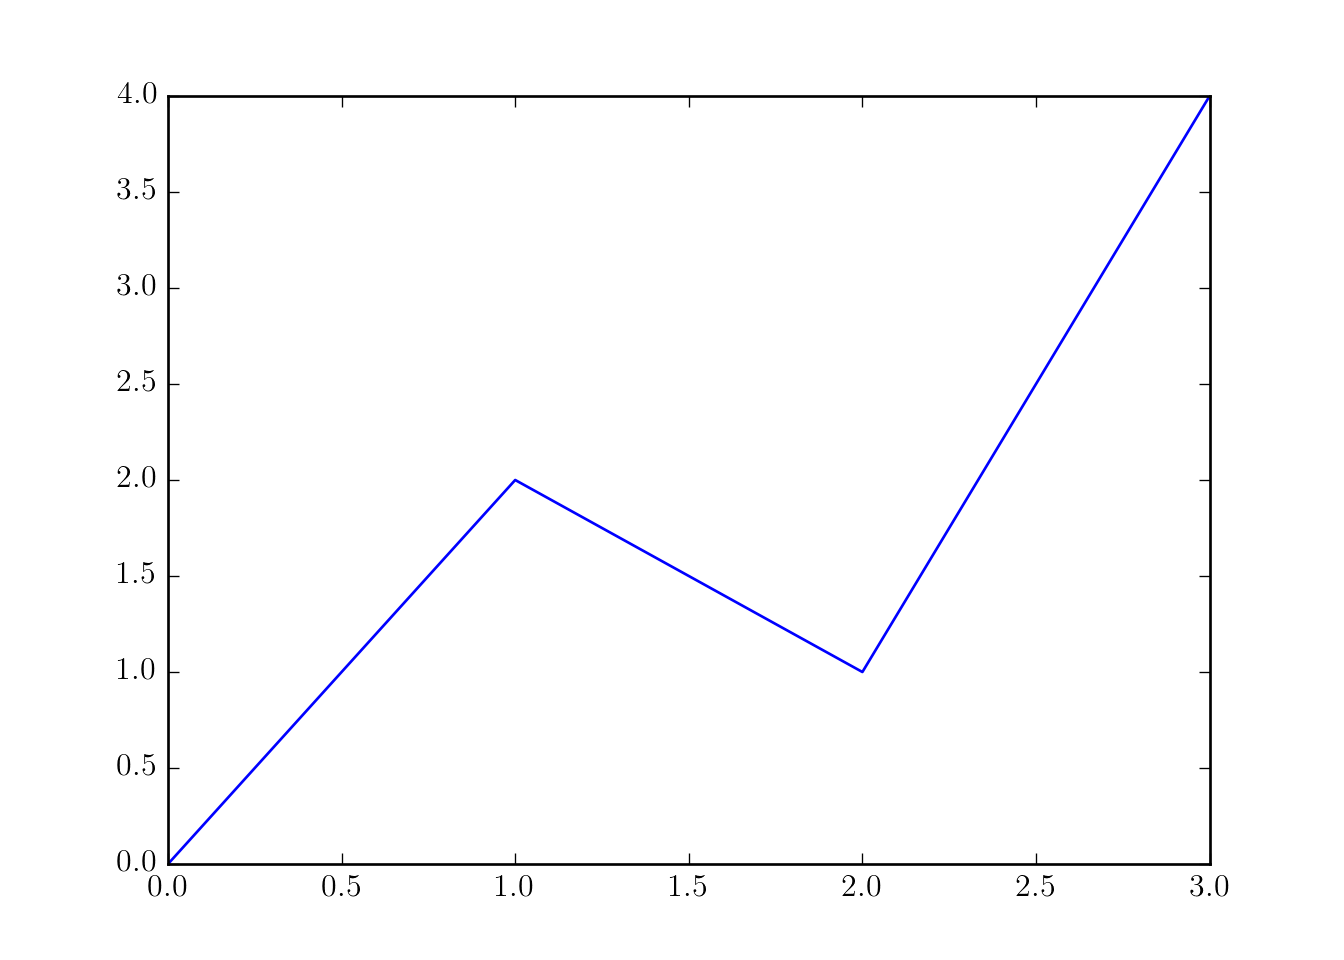
\includegraphics{/home/travis/build/markusmeister/travis-test/bookdown-demo_files/figure-latex/unnamed-chunk-11-1.pdf}

\bibliography{book.bib,packages.bib}

\end{document}
